\section{Design}
\label{sec:methodology}

% \wajih{Algorithm 2 (categorization) is cited as Algorithm 12 in some parts.}

% \wajih{Make sure you clarify this point at the revelant place in the design section. You probably also need to make it concise. "Central Server's Encryption Role: To clarify, the central server only generates the encryption key. It then distributes this key to the clients but does not perform any encryption or decryption operations on the semantic tokens themselves. This design prevents the central server from accessing the plaintext data. The central server does not possess the decryption key and therefore cannot decrypt the individual tokens. Its role is limited to key generation and distribution, ensuring it cannot access plaintext data."}


\begin{figure*}[t!]
  \centering
  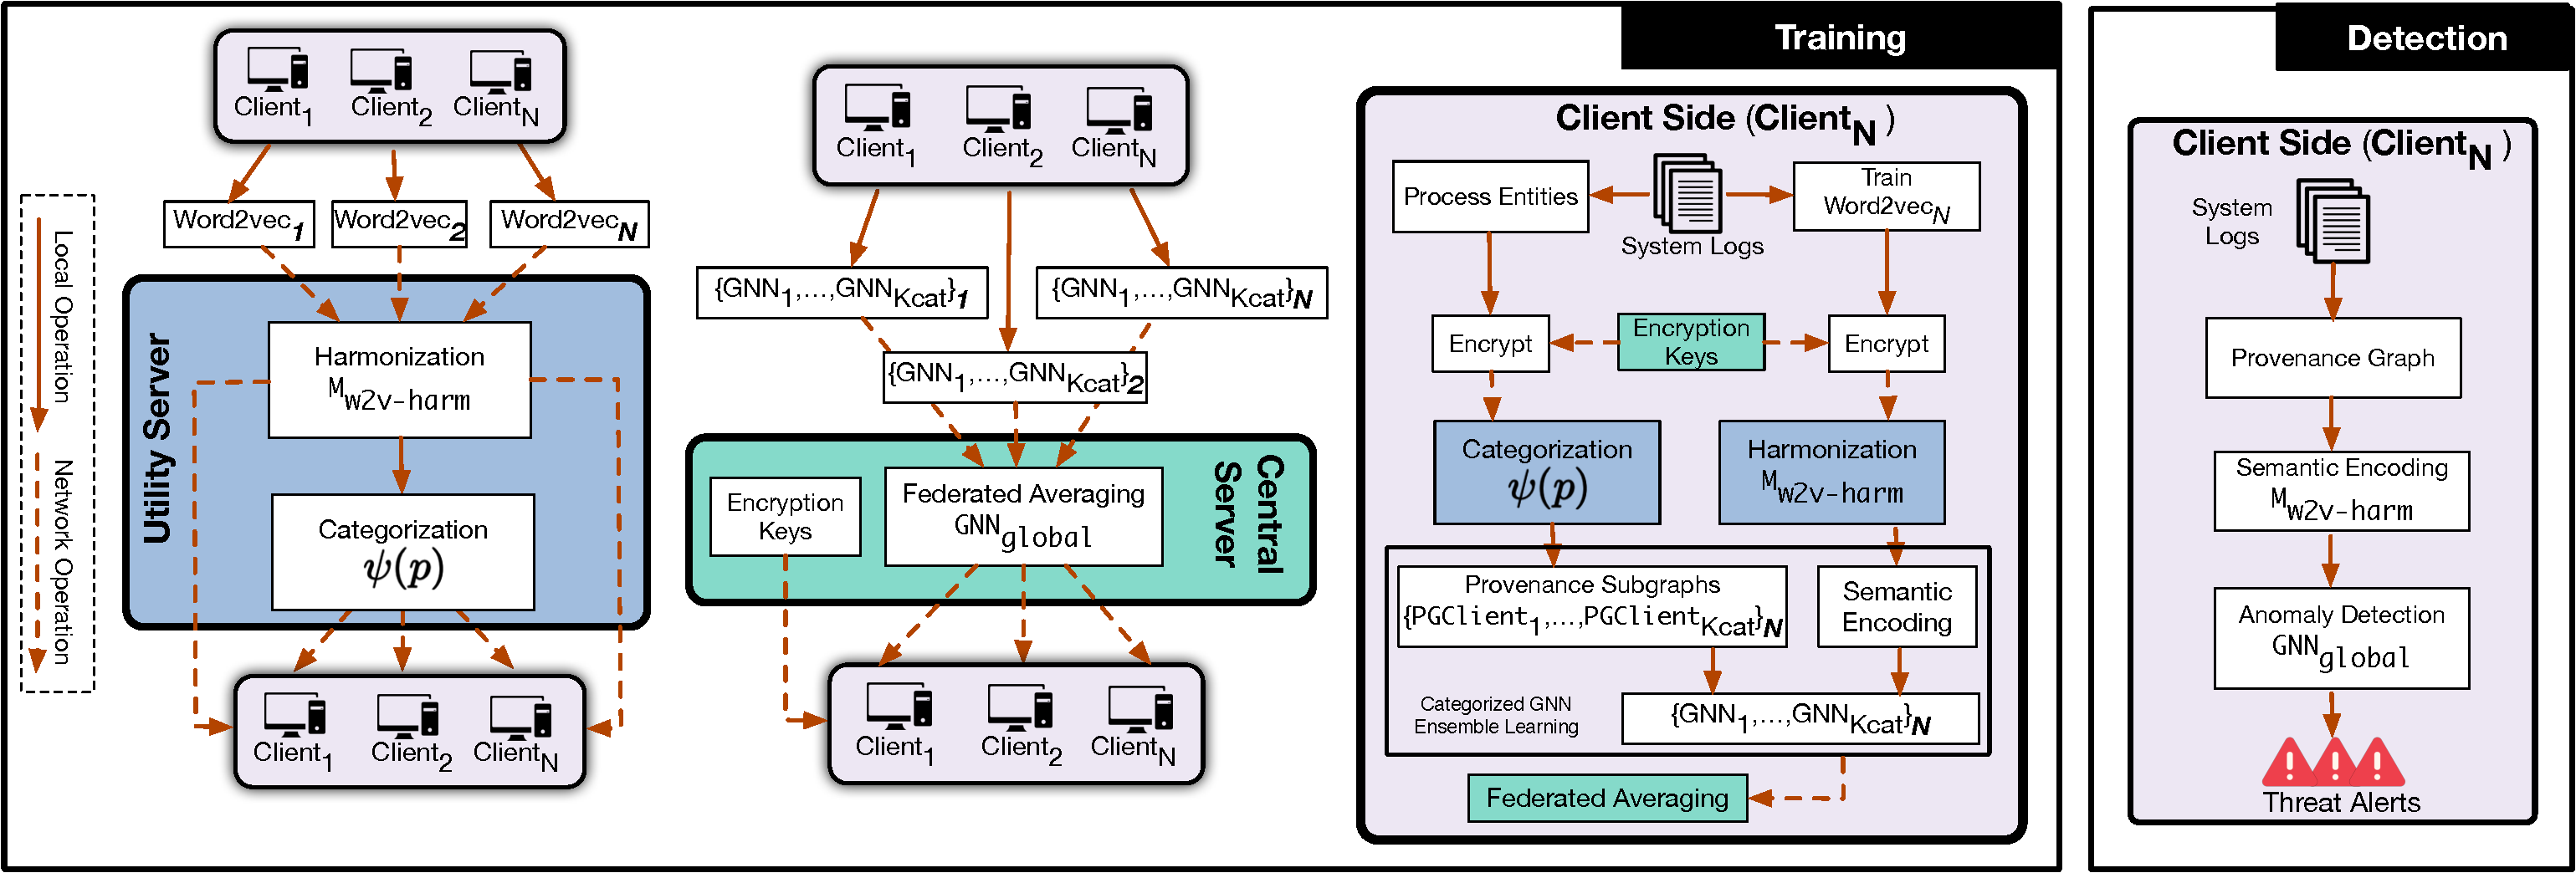
\includegraphics[width=1\textwidth]{fig/archv7.pdf}
  \caption{High-level architecture of \Sys. In the training phase, our system builds local provenance graphs for each client and trains an ensemble of \gnnshort models. Prior to this, we harmonize \wordvec models in a privacy preserving manner using encryption and dual-server architecture for semantic encoding. The local \gnnshort models participate in federated learning to develop a global \( {\text{GNN}}_{\text{global}} \) model, which is then utilized for anomaly detection. Notations are defined in Table~\ref{tab:keynotations}.}
  \vspace{-3ex}
  \label{fig:arch}
\end{figure*}


\subsection{Overview}
\Sys comprises six key components. Section~\ref{sub:provconstruct} builds provenance graphs from system logs on each client. Section~\ref{sub:word2vec:model} trains local \wordvec models to encode semantic attributes. Section~\ref{sub:model:harmonization} harmonizes these models using encryption and a utility server. Section~\ref{sys:catg} categorizes process entities across clients. Section~\ref{sys:fpgl} trains category-specific GNNs locally and aggregates them via federated learning. Section~\ref{sys:anomaly_detection} performs anomaly detection using the aggregated models. Figure~\ref{fig:arch} illustrates the architecture of \Sys.

\begin{table}[!t]
    \centering
    \scriptsize
    \caption{Key notations used in \Sys. \wajih{ Define  \( \Delta w_i \),   \( X_v \) }, \( v_k' \) }
    \label{tab:keynotations}
    \begin{tabular}{|p{3cm}|p{5cm}|}
    \hline
    \textbf{Notation} & \textbf{Definition} \\ \hline
    \( N \) & Total number of clients in federated learning. \\ \hline
    \( K_{cat} \) & Number of categories for process entities. \\ \hline
    \( \mathcal{C} = \{C_1, C_2, \ldots, C_N\} \) & Set of all client machines. \\ \hline
  
    \( PGClient_{i} = (\mathcal{V}_i, \mathcal{E}_i) \) & Provenance graph for client \( i \), with nodes \( \mathcal{V}_i \) and edges \( \mathcal{E}_i \). \\ \hline
    \( {GNN}_{\text{global}} = \{GNN_1, \ldots, GNN_{K_{cat}}\} \) & Set of global GNN models, one per category. \\ \hline
    \( w_j^{(r)} \) & Weights of global GNN for category \( j \) after round \( r \). \\ \hline
    \( \mathcal{P}_{\text{global}} \) & Global set of unique process entities. \\ \hline
    \( \psi(p) \) & Categorization map assigning process \( p \) to category \( \mathcal{C}_j \). \\ \hline
    \( y_v \) & True label of node \( v \). \\ \hline
    \( \hat{y}_v^j \) & Predicted label of node \( v \) by submodel \( j \). \\ \hline
    \( M_{\text{w2v-harm}} \) & Harmonized \wordvec model that converts contextual attributes into vector space. \\ \hline
    \( \mathcal{L}^{(r)} \) & Loss function value after round \( r \). \\ \hline
    \end{tabular}
  \end{table}

\begin{figure}[t!]
  \centering
  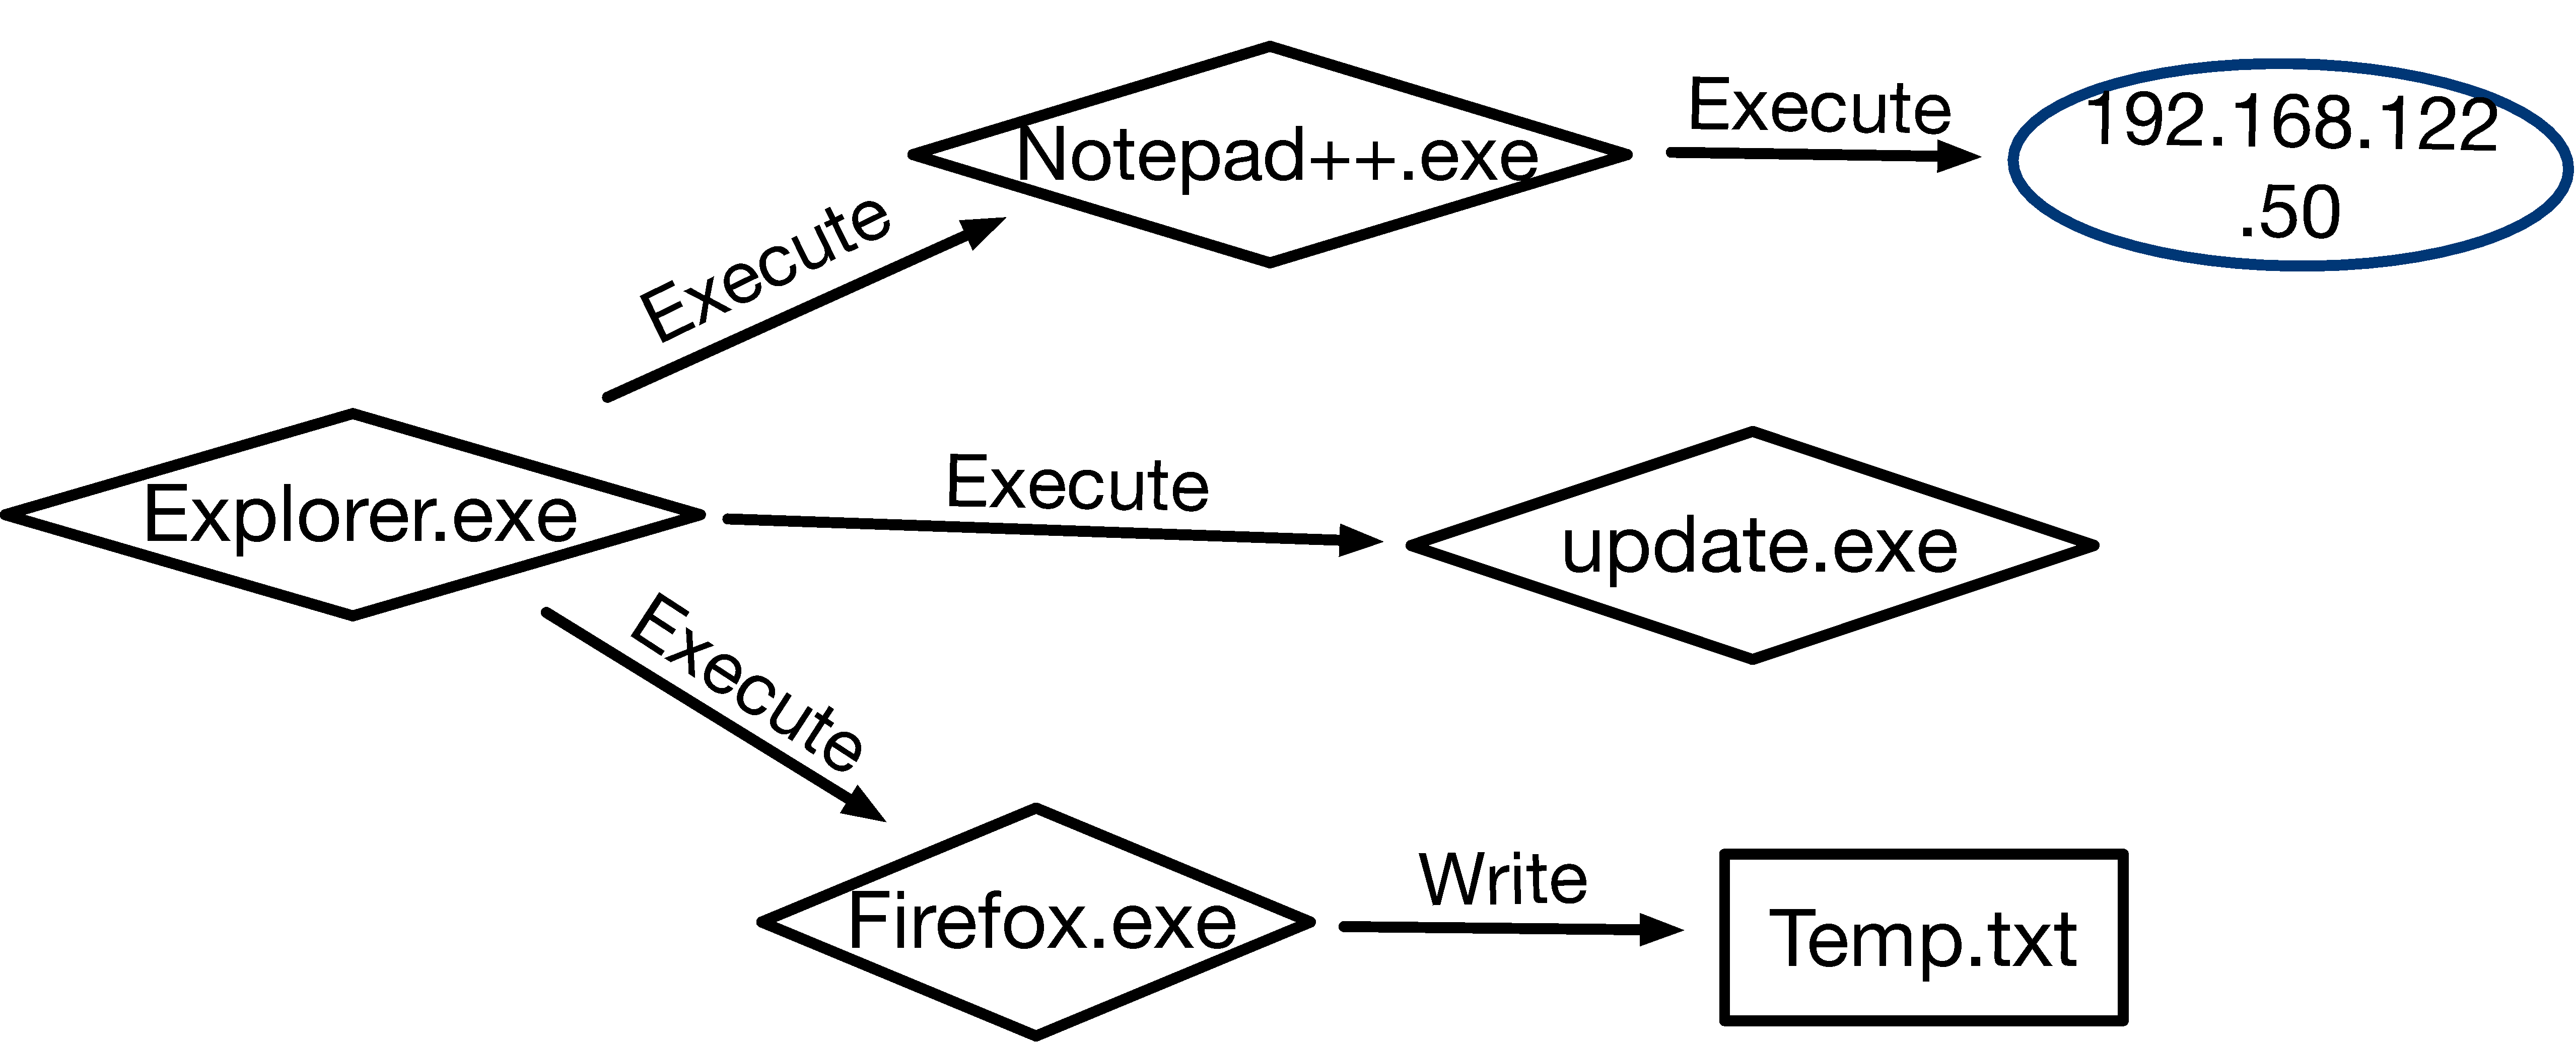
\includegraphics[width=0.4\textwidth]{fig/provexp.pdf}
  \caption{Data provenance graph example.}
  \label{provexp}
  \vspace{-3ex}
\end{figure}

\subsection{Problem Statement}
% \wajih{double check this subsection as I added this.}

\Sys aims to detect anomalous nodes in client-specific provenance graphs \( \{PGClient_{1}, PGClient_{2}, \ldots, PGClient_{N}\} \), which are constructed from system logs on a set of decentralized clients \( \mathcal{C} \). These anomalies represent deviations from benign behavior and are indicative of potential security threats.

To achieve this, \Sys employs a novel adaptation of Federated Learning (FL) to collaboratively train a set of global GNN models \( {GNN}_{\text{global}} = \{GNN_1, GNN_2, \ldots, GNN_{K_{cat}}\} \) without requiring raw log data to leave client machines. Each client locally optimizes its model by minimizing a loss function \( \mathcal{L}_i(w) \) and shares only model updates \( \Delta w_i \) with the central server. The global model is updated iteratively through aggregation: \( w = \frac{1}{N} \sum_{i=1}^{N} \Delta w_i, \)
where \( N \) represents the total number of clients. This decentralized approach preserves privacy while enabling the detection of threats across diverse and distributed system logs. The key notations for our system are summarized in Table~\ref{tab:keynotations}.



\subsection{Provenance Graph Constructor}
\label{sub:provconstruct}

\Sys builds a system provenance graph on each client using local \logs. It leverages built-in logging tools, such as Linux Audit~\cite{linuxaudit}, which record detailed system activities. These include process executions, file accesses, and network events. \Sys constructs a graph where nodes represent entities like processes, files, and sockets. Edges correspond to syscalls capturing interactions between them. Each node is enriched with attributes such as process names, command lines, file names, and IP addresses. Prior work~\cite{flash2024,cheng2023kairos} shows these attributes help the model learn normal system behavior. Figure~\ref{provexp} illustrates a graph where \textit{Explorer.exe} spawns processes like \textit{Notepad.exe} and \textit{Firefox.exe}, which interact with file and socket nodes.



\subsection{\wordvec Model Generation}
\label{sub:word2vec:model}

After each client machine \(C_i\in \mathcal{C}\) generates its local provenance graph \(PGClient_{i} = (\mathcal{V}_i, \mathcal{E}_i)\), the node attributes in \(\mathcal{V}_i\) are converted into feature vectors for the subsequent graph learning phase. Existing systems, such as \flash~\cite{flash2024}, have demonstrated the effectiveness of leveraging semantic attributes of nodes to enhance detection performance. System logs contain rich attributes associated with various entities, including process names, file paths, and network IP addresses. These attributes must be transformed into vector space to serve as node features for the global GNN models.

For this encoding, we employ the \wordvec~model which processes different semantic attributes based on node types:
\begin{itemize}[itemsep=0.1em, parsep=0em, topsep=0em, leftmargin=*]
    \item \textbf{Process:} Process name and command-line arguments.
    \item \textbf{File:} File path.
    \item \textbf{Socket:} IP addresses and port.
\end{itemize}


  

For each node \(v \in \mathcal{V}_i\), we extract its 1-hop subgraph by collecting all neighbors of \(v\). We transform this node subgraph into a ``document'' by combining:
\begin{enumerate}[itemsep=0.1em, parsep=0em, topsep=0em, leftmargin=*]
    \item The semantic attributes of \(v\).
    \item The types of causal events captured along the edges.
    \item The relevant attributes of its neighbor nodes.
\end{enumerate}

These node-centric documents are then encoded into fixed-length vectors via \wordvec, which is trained on benign system logs. This approach effectively captures the semantic relationships between terms, producing dense embeddings that serve as node features for graph representation learning.

\subsection{Privacy-preserving Model Harmonization}
\label{sub:model:harmonization}



\PP{Addressing Token Variability Across Clients}
Each client independently trains a \wordvec model using their local logs for feature encoding. However, before these models can be utilized to encode text attributes effectively, it is essential to contextually merge individual client \wordvec models into a unified model \( M_{\text{w2v-harm}} \) for use across all clients. This unification is crucial; without it, each client would produce a different encoding, \(v_a^i\), for identical inputs, where \(i\) denotes the client. The variability in feature vectors, \(\{v_a^1, v_a^2, \ldots, v_a^N\}\), for the same attribute \(a\) across \(N\) clients, would compromise the consistency of client-based \gnnshort models. To ensure uniformity, the feature vectors for overlapping attributes must be averaged across clients. Such averaging ensures consistency in the feature representation, enhancing the effectiveness of the federated averaging technique by maintaining uniformity in the input space for the \gnnshort models across all clients.

Our system harmonizes only the tokens that overlap in the \wordvec models across clients. Tokens that do not overlap are not averaged and remain unchanged. While clients share common activities due to standard system-level routines, some variations and patterns are unique to each client. Non-overlapping tokens preserve these unique patterns; however, they contribute to additional heterogeneity, which cannot be eliminated through harmonization. If these unique patterns are not accurately learned, they can lead to high false alarm rates. To capture these distinct local variations between clients, we have developed a novel ensemble GNN learning framework, detailed in Section~\ref{sys:fpgl}, where each submodel specializes in distinct system patterns across clients, enhancing model precision as shown in Section~\ref{sec:eval}.
\emph{To better understand the degree of overlap in real-world settings, we now turn to an examination of client token overlap statistics.}

%\wajih{Let's handle this comment as well "For "Overlap Statistics Across Clients.", I guess the authors compute the numbers on 0-hop node (no neighborhood information is used), but the Word2Vec aggregation is based on 1-hop. "}

\begin{algorithm}[!t]
    \scriptsize
    \DontPrintSemicolon
    \SetKwInOut{Input}{Inputs}
    \SetKwInOut{Output}{Output}
    \Input{Client Word2Vec models $\{Word2vec_1, Word2vec_2, \ldots, Word2vec_N\}$.}
    \Output{Harmonized Word2Vec model $M_{\text{w2v-harm}}$ sent to clients.}
    \BlankLine
    \tcc{Central server distribute symmetric encryption keys to each client.}
    \ForEach{client $C_i$}{
  
      Send $key$ to $C_i$\\
    }
    \tcc{Clients encrypt their model tokens.}
    \ForEach{client model $word2vec_i$}{
      $Word2vec_i \leftarrow$ EncryptModelTokens($Word2vec_i$, $E$) \tcc*{Encrypt tokens using $E$.}
      Send $Wor2vec_i$ to Utility Server\\
    }
    \tcc{Utility server merges encrypted models.}
    $TokenVectors \leftarrow$ InitializeEmptyDictionary()\\
    $TokenCounts \leftarrow$ InitializeEmptyDictionary()\\
    \ForEach{encrypted model $Word2vec_i$}{
      \ForEach{token $t$ in $Word2vec_i$}{
        $Vector \leftarrow Word2vec_i[t]$\\
        \eIf{$TokenVectors$.HasKey($t$)}{
          $TokenVectors[t] \leftarrow TokenVectors[t] + Vector$\\
          $TokenCounts[t] \leftarrow TokenCounts[t] + 1$\\
        }{
          $TokenVectors[t] \leftarrow Vector$\\
          $TokenCounts[t] \leftarrow 1$\\
        }
      }
    }
    \tcc{Average the vectors for overlapping tokens.}
    \ForEach{token $t$ in $TokenVectors$.Keys()}{
      $TokenVectors[t] \leftarrow TokenVectors[t] / TokenCounts[t]$\\
    }
    $M_{\text{w2v-harm}} \leftarrow$ NewModel($TokenVectors$, $EncryptedTokens$) \tcc*{Constructing a new harmonized model.}
    \ForEach{client $C_i$}{
      Send $M_{\text{w2v-harm}}$ to $C_i$\\
    }
    \BlankLine
    \Return{Harmonized model $M_{\text{w2v-harm}}$ has been dispatched to all clients.}\\
    \BlankLine
    \caption{Privacy-preserving \wordvec Model Harmonization.}
    \label{alg:secure_integration_averaging_word2vec}
  \end{algorithm}
\PP{Overlap Statistics Across Clients}
Our experiments with the \optc dataset revealed that, on average, different hosts can have up to 75\% overlap in process names, 41\% in files, and 60\% in network flows in the system logs. This finding aligns with related work \cite{flash2024}, which shows that many system-level processes and files are common across different systems. In a centralized \pids, these attributes are learned by a single semantic model, mapping them to the same embedding space. In contrast, a federated setting, where each client trains its own model, can introduce model bias into the token embeddings, complicating the convergence for downstream GNN models using these vectors. To address this, it is essential to harmonize overlapping tokens to provide the model with a unified understanding of the semantic information present in system logs.
\emph{However, to achieve this harmonization securely and without compromising user privacy, we employ an encryption-based strategy, as described next.}

\PP{Harmonization with Encryption}
Transferring tokens, containing sensitive data like process names, file names, and IP addresses, to a central server could breach user privacy. To mitigate this, we employ a trusted utility server. Initially, the central server uses Fernet symmetric key encryption~\cite{ismail2020fernet,bokhari2016review} to generate an encryption key, which is distributed to clients. Clients then encrypt their \wordvec model tokens using the encryption key: \(E(v_{k}) = v_{k}^{'}\) and send them to the utility server. This server merges the encrypted models and dispatches the unified semantic vectors back to the respective clients, who decrypt them back: \(D(v_{k}^{'}) = v_{k}.\) This procedure ensures that neither the central server nor the utility server can access the actual token information, assuming no collusion between the two servers. The process is detailed in Algorithm~\ref{alg:secure_integration_averaging_word2vec}.



\subsection{Process Entity Categorization}
\label{sys:catg}

% \wajih{This is section difficult to absorb. So let's make figure for the workflow. In the figure we will clarify how processes from different clients are collected, categorized into Kcat bins, and redistributed. In the figure have two Client A and Client B each send encrypted process names. Utility server merges them into Pglobal. Randomly assigns categories via Phi (p). Sends category mappings back to clients. Clients form per-category bins. Use consistent terminology. I am expecting a Flowchart-style with arrows and category bins.}

\begin{figure}[t!]
    \centering
    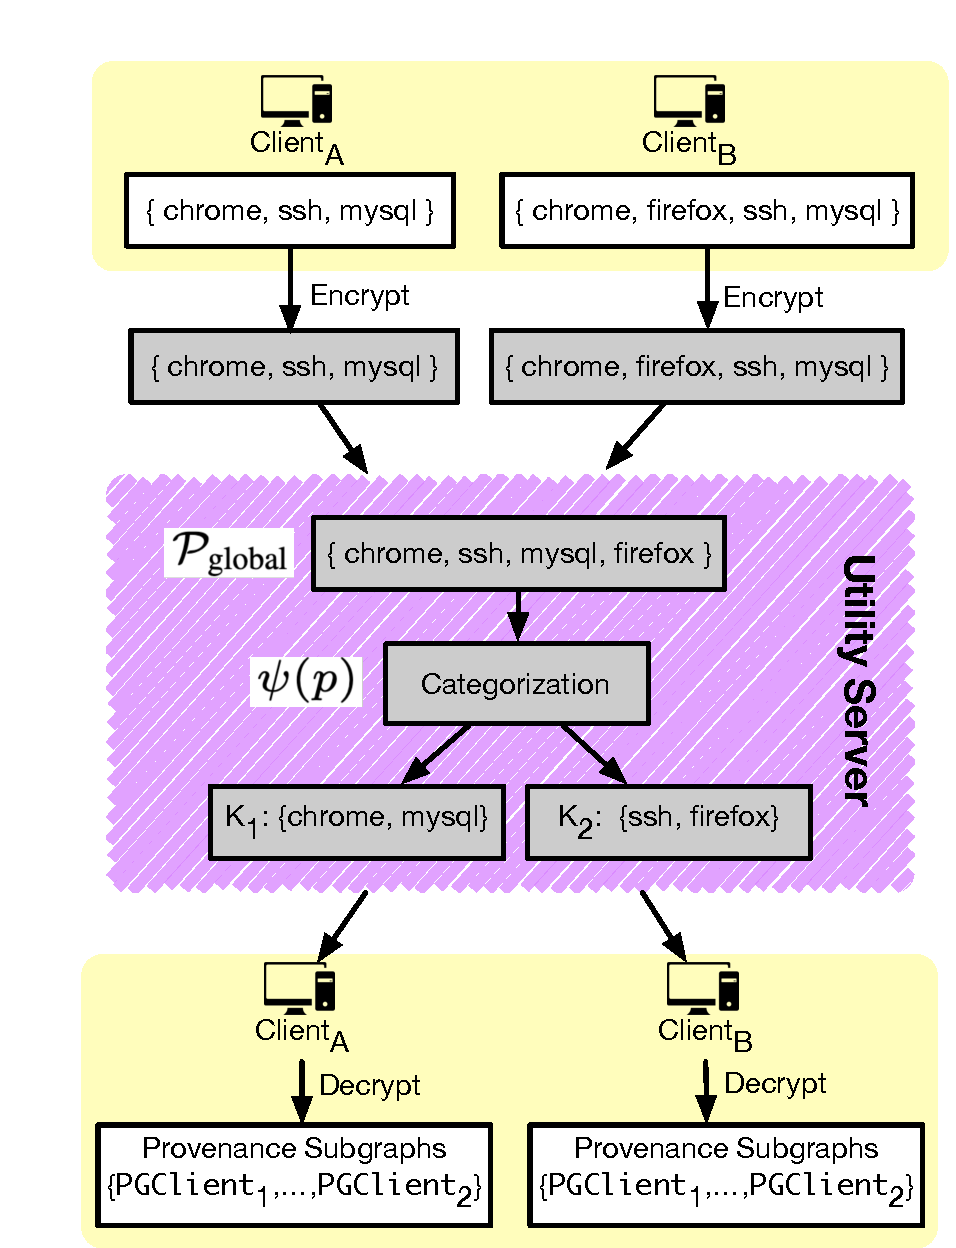
\includegraphics[width=0.4\textwidth]{fig/categorization_flow.pdf}
    \caption{Secure process entity categorization workflow: Clients encrypt their process names and send them to the utility server, which categorizes them into bins and sends the results back. The clients then generate a provenance subgraph for each bin to support \gnnshort ensemble learning. \Fix{Grey boxes represent encrypted.}}
    \label{proc:cate}
    \vspace{-3ex}
  \end{figure}

During our initial experiments (Table~\ref{categorized_gnn}), we found that a single \( {GNN}_{\text{global}} \) cannot achieve good detection performance in an FL setting due to the diverse and heterogeneous distributions of clients data. The disparity in data distributions among \( N \) clients poses a significant challenge in effectively training a unified model that can generalize well across all clients, since the global model struggles to capture the unique characteristics and patterns inherent in each client's data. To address this limitation, we developed a comprehensive framework that organizes process entities across different clients into distinct groups. Each category is modeled by a dedicated submodel, enabling it to focus on the unique distribution and intricate patterns of its assigned category and thereby enhance overall detection performance.

% \wajih{please refer to algorithm in the whole paragraph. Divide the following paragraph into three steps using latex enumerate macro.}
The framework leverages a central utility server to orchestrate the categorization of process entities. Specifically, it proceeds in three main steps:
\begin{enumerate}[itemsep=0.1em, parsep=0em, topsep=0em, leftmargin=*]
    \item \textbf{Collection of Encrypted Process Names.} Each client \(C_i \in \mathcal{C}\) transmits an encrypted list of its process names to the utility server. The server merges these into a global list of unique process entities, denoted by \( \mathcal{P}_{\text{global}} \).

    \item \textbf{Random Categorization.} The utility server applies the categorization map \( \psi(p) \) to randomly partition all process names in \( \mathcal{P}_{\text{global}} \) into \( K_{cat} \) categories. Although the partitioning is random, it is performed only once at the global level, ensuring that any process name \( p \) is consistently mapped to the same category \( j \) across all clients, i.e., \( \psi(p) = j \).

    \item \textbf{Distribution of Categories.} Finally, the resulting category assignments are disseminated back to each client, guaranteeing a unified and consistent mapping of processes into categorized bins across the federated network.
\end{enumerate}

% Once the categories are established, each client employs the categorized process sets to build provenance subgraphs \( PGClient_{i} \). The neighborhood hop length of these subgraphs is aligned with the number of graph convolution layers in \( {GNN}_{\text{global}} \), ensuring the model has complete neighborhood information for each node. In our experiments, we fix this hop length to two, which past studies~\cite{wang2022threatrace,flash2024} have shown to offer an optimal trade-off between efficiency and accuracy. These subgraphs provide training data for an ensemble of \({GNN}_{\text{global}}\) models in a federated manner. Each submodel specializes in learning the patterns of its assigned category and participates in federated averaging. This ensures a balanced segmentation of data across clients and maintains consistency in the training datasets for each submodel before federated averaging.

% \wajih{move this example at the of this subsection. Make sure that transitions among all the paragraphs is smooth.}
Figure~\ref{proc:cate} illustrates this with an example. The categorization process divides the overall learning task into sub-tasks (submodels) by distributing them into different subsets of processes across clients in a standardized manner. As a result, the influence of clients with larger datasets is spread across multiple models. This approach reduces the risk of any single client dominating the federated learning process and promotes more balanced contributions from all participants, ultimately enhancing the system's robustness and performance.
%consider two clients: \emph{A} and \emph{B}:
% \begin{itemize}[itemsep=0.1em, parsep=0em, topsep=0em, leftmargin=*]
%     \item \emph{A} has a set of processes \{\texttt{chrome}, \texttt{ssh}, \texttt{mysql}\}.
%     \item \emph{B} has a set of processes \{\texttt{chrome}, \texttt{firefox}, \texttt{ssh}, \texttt{mysql}\}.
% \end{itemize}
% Both clients send encrypted lists of these process names to the utility server, which combines them into a single global list of unique names \{\texttt{chrome}, \texttt{ssh}, \texttt{mysql}, \texttt{firefox}\}. The server then applies \( \psi \) to randomly assign each name to one of the \( K_{cat} \) categories. For example, \( \psi(\texttt{chrome}) \) and \( \psi(\texttt{mysql}) \) may map to category~1, while \( \psi(\texttt{ssh}) \) and \( \psi(\texttt{firefox}) \) map to category~2.

% This assignment is transmitted back to both clients, ensuring that \texttt{chrome} and \texttt{mysql} are consistently grouped under category~1, and \texttt{ssh} and \texttt{firefox} under category~2. As a result, each category gathers similar processes across all clients, even though the initial split is random. By dividing the overall task into sub-tasks (submodels) and distributing them to different subsets of processes, the influence of clients with larger datasets is shared among multiple models. This approach reduces the risk of any single client dominating the federated training process and facilitates more balanced contributions from all participants, ultimately improving the robustness and performance of the system.

%\begin{algorithm}[!t]
    \scriptsize
    \DontPrintSemicolon
    \SetKwInOut{Input}{Inputs}
    \SetKwInOut{Output}{Output}
    \caption{Categorizing processes into \(\,K_{cat}\) categories.}
    \label{alg:categorization_process}
  
    \Input{
      Number of clients \(N\); Number of categories \(K_{cat}\); Client datasets \(\mathcal{C}\)
    }
    \Output{
      Category assignment function \(\psi\)
    }
  
    \BlankLine
    \tcc{Step 1: Initialization of utility server and global process list.}
    \(\mathcal{P}_{\text{global}} \leftarrow \emptyset\) \\
    \ForEach{client \(C_i \in \mathcal{C}\)}{
        Transmit encrypted process list to utility server \\
        \(\mathcal{P}_{\text{global}} \leftarrow \mathcal{P}_{\text{global}} \cup \text{Encrypt}(C_i)\)
    }
  
    \BlankLine
    \tcc{Step 2: Categorization of processes into \(K_{cat}\) categories.}
    \For{\(p \in \mathcal{P}_{\text{global}}\)}{
        \(\psi(p) \leftarrow \text{RandomCategory}(K_{cat})\)
    }
  
    \BlankLine
    \tcc{Step 3: Distribute global category assignments to clients.}
    \ForEach{client \(C_i \in \mathcal{C}\)}{
        Send categorization \(\psi\) to \(C_i\)
    }
  
    \BlankLine
    \Return \(\psi\)
    \label{alg:categories}
  \end{algorithm}

\subsection{FL with Categorized GNN Ensemble Learning}
\label{sys:fpgl}



% \wajih{First paragraph should connect this subsection with the previous subsection. Say something like "Once the blah blah is generated in the previous module (Section{}), we can use these blah blah for blah blah. However, blah blah is not possible without blah blah.}

%\wajih{Is process entitiy categorization related to Categorized Provnenace subgraph? it is not clear at all. Please do not use words without connecting them with the broader context.}

% \wajih{move this paragraph to discussion section why we combine FL with GNN.}
% APTs involve multiple causally linked attack steps across various system entities, highlighting the need to capture and model the interactions among these entities for effective detection. Analyzing each system event in isolation does not allow us to capture these interactions properly, as observed in existing log-level systems~\cite{deeplog2017,liu2019log2vec,xia2019loggan}; hence, provenance graphs, \( PGClient_{i} \), are being used to effectively model the interaction of system entities. Moreover, graph representation learning is used to learn the patterns present in these graphs, as shown in related works~\cite{flash2024,cheng2023kairos,jia2023magic}. We integrate federated learning with graph representation learning to bring privacy and decentralization to intrusion detection while maintaining the strong detection performance offered by the provenance graph learning technique.

% \wajih{Refer to the Algorithm throught the paragraph. use steps just like you have in the algorithm. Maybe break this paragraph into multiple paragraph otherwise this subsection will look very small. }
% Our approach includes a central server responsible for initializing the global GNN models, \({GNN}_{\text{global}}\), with random weights, \( w_j^{(0)} \), which are then sent to all clients in \( \mathcal{C} \). These clients use their local process subgraphs, \( PGClient_{i} \), and semantic feature vectors to train the GNN models in an unsupervised way, following a training method similar to \flash. The objective of the GNN model is to classify each node \( v \) into its corresponding type, yielding predictions \(\hat{y}_v^j\). The server then applies the federated averaging algorithm to merge the GNN models into a set of global models, \({GNN}_{\text{global}}\), based on the process entity categories on which they were trained. This ensures that models with similar distributions are combined together to address the data heterogeneity problem. Specifically, the server aggregates parameters from \( N \) client models to update each global submodel as \(\bar{w} = \frac{1}{N} \sum_{i=1}^{N} w_i\). Algorithm~\ref{alg:training_submodel} explains this process in detail.

% The federated averaging process is repeated for a set number of rounds \( R \), and concludes when there is no further reduction in the training loss, \(\mathcal{L}^{(r)}\). 

Once the categorized bins of processes have been generated, we train specialized GNN models for each bin. Each \({GNN}_{\text{global}}\) submodel focuses on a standardized subset of processes across clients, identified through entity categorization. This approach effectively captures distinct patterns and structures while reducing data heterogeneity. Our method proceeds in three main steps, as detailed in Algorithm~\ref{alg:training_submodel}.

\textbf{Step 1: Initialization.} As in Step~1 of Algorithm~\ref{alg:training_submodel}, the central server initializes the global GNN models, \({GNN}_{\text{global}}\), with random weights \( w_j^{(0)} \). The server then transmits these initial weights \( w_j^{(0)} \) to all clients in \(\mathcal{C}\).

\textbf{Step 2: Local Model Training.} Each client \( C_i \) organizes its local processes into bins based on the assigned categories, \(\psi(p)\) which it gets using the methodology detailed in section~\ref{sys:catg}. From each category bin, the client constructs a \emph{provenance subgraph} capturing the local relationships of processes within that category. The neighborhood hop length of these subgraphs matches the number of graph convolution layers in \({GNN}_{\text{global}}\), ensuring the model has sufficient neighborhood information for each node. Each client then leverages these categorized subgraphs, along with semantic feature vectors, to train the GNN models in an unsupervised manner. Similar to the approach in \flash, the objective of each GNN submodel is to classify every node \(v\) into its corresponding type, yielding predictions \(\hat{y}_v^j\). This localized, category-focused training ensures that each submodel effectively captures the unique structures and distributions within each category for the client’s data.

\textbf{Step 3: Federated Averaging and Category-Based Aggregation.} As in Step~2 of Algorithm~\ref{alg:training_submodel}, the server collects the updated parameters from all \( N \) clients for each category-specific submodel. It then applies the federated averaging algorithm to merge these parameters, computing \( \bar{w} \;=\; \frac{1}{N} \sum_{i=1}^{N} w_i \)
for each category’s global submodel. Because every submodel is trained on processes belonging to the same category across all clients, the data distributions within each submodel are more homogeneous, effectively addressing data heterogeneity. This category-based aggregation integrates knowledge gained from multiple clients, leading to robust, specialized global models. It is important to note that the central server receives only the model weights from clients; no raw system log data is transmitted to it.

The federated averaging process (Step~3 of Algorithm~\ref{alg:training_submodel}) is repeated for \( R \) rounds, concluding once there is no further reduction in the training loss \(\mathcal{L}^{(r)}\). The resulting ensemble of global submodels, each attuned to a distinct process category, provides a comprehensive solution that balances the diverse data distributions across clients while preserving privacy.

\begin{algorithm}[!t]
    \scriptsize
    \DontPrintSemicolon
    \SetKwInOut{Input}{Inputs}
    \SetKwInOut{Output}{Output}
    \caption{Training and federated aggregation of category-specific submodels.}
    \label{alg:training_submodel}
  
    \Input{
      Global process list \(\mathcal{P}_{\text{global}}\), \\
      Category assignment function \(\psi\), \\
      Number of categories \(K_{cat}\), \\
      Client datasets \(\mathcal{C}\)
    }
    \Output{
      Trained global GNN models \(\text{GNN}_{\text{global}}\)
    }
  
    \BlankLine
    \tcc{Step 1: Local training of submodels for each category.}
    \ForEach{client \(C_i \in \mathcal{C}\)}{
        \ForEach{\(p \in C_i\)}{
            \(j \leftarrow \psi(p)\) \\
            Train GNN submodel on processes in category \(j\) from client \(C_i\)
        }
    }
  
    \BlankLine
    \tcc{Step 2: Aggregation and federated averaging of submodels.}
    \ForEach{category \(j \in \{1, \ldots, K_{cat}\}\)}{
        \(w_j^{(0)} \leftarrow \text{InitializeRandomWeights}()\) \\
        \ForEach{client \(C_i \in \mathcal{C}\)}{
            \(w_j^{(i)} \leftarrow \text{ExtractWeights}(C_i, j)\)
        }
        \(\displaystyle w_j^{(r)} \leftarrow \text{FederatedAveraging}\bigl(\{w_j^{(i)}\}\bigr)\)
    }
  
    \BlankLine
    \Return \(\displaystyle \text{GNN}_{\text{global}} \leftarrow \{\,w_1^{(r)},\, w_2^{(r)},\, \ldots,\, w_{K_{cat}}^{(r)}\}\)
    \label{alg:submodel}
  \end{algorithm}
  

\subsection{GNN-based Anomaly Detection}
\label{sys:anomaly_detection}

\Sys employs a node level detection methodology focusing on identifying irregular nodes through the comparison of their expected and observed types. This approach is grounded in a detailed analysis of both the surrounding structures and inherent properties of the nodes, to define normal pattern baselines for various node types. Typically, entities with malicious intentions display neighborhood structures and characteristics deviating from these established norms as shown in previous work~\cite{flash2024,cheng2023kairos,yangprographer}. In operational phases, the detection of anomalies that diverge from the pre-established node distribution patterns often results in their misclassification. The emergence of nodes misclassified in the system's output is indicative of potential security issues.

\Sys performs threat detection in a decentralized manner on clients' provenance graphs (\( \{PGClient_{1}, PGClient_{2}, \ldots, \\ PGClient_{N}\} \)) in an organization. For a given provenance graph \(PGClient_{i}\), \Sys uses the \( {GNN}_{\text{global}} \) \(\{GNN_1, \\ GNN_2, \ldots, GNN_{K_{cat}}\}\) trained using federated learning. Each submodel performs inference on the client's full provenance graph, utilizing the nodes' features \(X_v\) and the graph's adjacency matrix \(A\) to predict each node \(v\)'s label \(\hat{y}_v^j\). Let us define a misclassification indicator \(\mathcal{M}(v, j)\) as
\[
\mathcal{M}(v, j) \;=\;
\begin{cases}
1, & \text{if } \hat{y}_v^j \neq y_v,\\
0, & \text{otherwise}.
\end{cases}
\]
Accordingly, a node \(v\) is identified as an anomaly if it is misclassified by \emph{all} submodels, i.e.,
\[
\mathcal{A}(v) \;=\;
\begin{cases}
1, & \text{if } \sum_{j=1}^{K_{cat}} \mathcal{M}(v, j) \;=\; K_{cat},\\
0, & \text{otherwise}.
\end{cases}
\]
This indicates that none of the submodels recognize the neighborhood structure or features displayed by \(v\), prompting its classification as an anomaly. To regulate the frequency of alerts, we define a threshold \(T\) similar to \flash. This parameter sets a threshold on the likelihood of a classification being considered valid, with a higher value of \(T\) implying stronger confidence and increasing the probability of identifying anomalies.
